\documentclass[12pt, twoside]{article}
\usepackage[letterpaper, margin=1in, headsep=0.5in]{geometry}
\usepackage[english]{babel}
\usepackage[utf8]{inputenc}
\usepackage{amsmath}
\usepackage{amsfonts}
\usepackage{amssymb}
\usepackage{tikz}
\usetikzlibrary{quotes, angles}
\usepackage{graphicx}
%\usepackage{pgfplots}
%\pgfplotsset{width=10cm,compat=1.9}
%\usepgfplotslibrary{statistics}
%\usepackage{pgfplotstable}
%\usepackage{tkz-fct}
%\usepackage{venndiagram}

\usepackage{fancyhdr}
\pagestyle{fancy}
\fancyhf{}
\renewcommand{\headrulewidth}{0pt} % disable the underline of the header

\fancyhead[RE]{\thepage}
\fancyhead[RO]{\thepage \\ Name: \hspace{3cm}}
\fancyhead[L]{BECA / Dr. Huson / Geometry 10th Grade\\* Unit 2: Midpoints and distance \\ 
25 September 2019}

\begin{document}
  \subsubsection*{2.7 Re-Quiz: Segment \& Area Calculations}

  \begin{enumerate}
    \item Complete the construction of an equilateral triangle with one side as $\overline{AB}$. \vspace{6cm}
    \begin{center}
    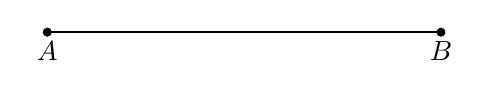
\begin{tikzpicture}
      \draw [-, thick] (0,0)--(5,0);
      \draw [fill] (0,0) circle [radius=0.05] node[below]{$A$};
      \draw [fill] (5,0) circle [radius=0.05] node[below]{$B$};
    \end{tikzpicture}
    \end{center} \vspace{6cm}

    \item Given $\overleftrightarrow{RS}$ as shown on the number line. \\[20pt] % Midpoint
    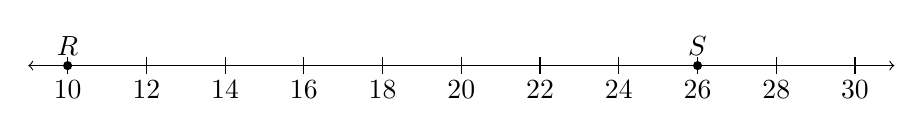
\begin{tikzpicture}[scale=0.5]
      \draw [<->] (9,0)--(31,0);
      \foreach \x in {10, 12,...,30} %2 leading for diff!=1
        \draw[shift={(\x,0)},color=black] (0pt,-6pt) -- (0pt,6pt) node[below=5pt]  {$\x$};
        \draw [fill] (10,0) circle [radius=0.1] node[above] {$R$};
        \draw [fill] (26,0) circle [radius=0.1] node[above] {$S$};
    \end{tikzpicture} \\[20pt]
    Mark and label the point $M$ that bisects $\overline{RS}$.

\newpage

\item Find the area of $\triangle ABC$. The altitude $h$ of the triangle is $4 \frac{3}{4}$ centimeters and the base $AB=9 \frac{1}{2}$ cm. (diagram not to scale) \\[0.5cm]
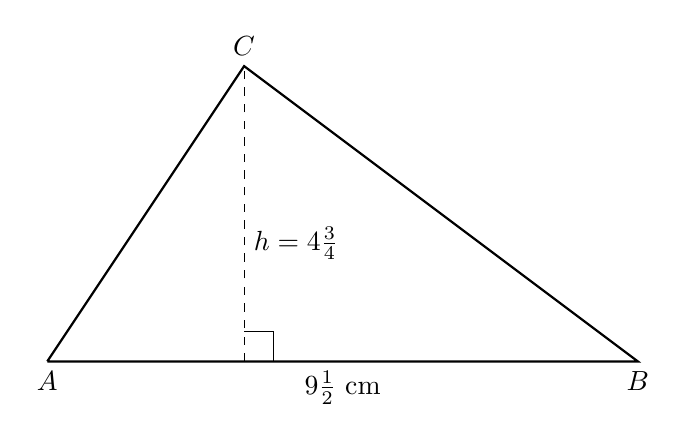
\begin{tikzpicture}[scale=1.25]
  \draw [thick]
    (2,0)node[below]{$A$}--
    (8,0)node[below]{$B$}--
    (4,3)node[above]{$C$} --(2,0);
 \draw [dashed] (4,0)--(4,3);
 \draw (4,0)++(0.3,0)--++(0,0.3)--+(-0.3,0);
 \node at (4,1.2)[right]{$h=4 \frac{3}{4}$};
 \node at (5,0)[below]{$9 \frac{1}{2}$ cm};
\end{tikzpicture} \vspace{1.0cm}

\item Given $\overline{PQRS}$, $PQ=3 \frac{1}{4}$, $QR=1 \frac{1}{4}$, and $RS= 5 \frac{1}{2}$. (diagram not to scale)\\ [0.25cm]
  Find ${PS}$.\\[.5in]
      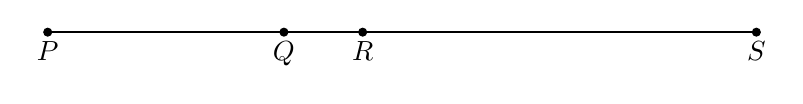
\begin{tikzpicture}
        \draw [-, thick] (0,0)--(9,0);
        \draw [fill] (0,0) circle [radius=0.05] node[below]{$P$};
        \draw [fill] (3,0) circle [radius=0.05] node[below]{$Q$};
        \draw [fill] (4,0) circle [radius=0.05] node[below]{$R$};
        \draw [fill] (9,0) circle [radius=0.05] node[below]{$S$};
      \end{tikzpicture}
      \vspace{3cm}

\item Given that $M$ is the midpoint of $\overline{AB}$. $AM=7x+4$, $BM=5x+8$. Find ${AB}$.\\
Complete all the steps for full credit (including a fully-labeled drawing and the check)

\end{enumerate}
\end{document}
